%-------------------------------------------------------------%
% Dissertation template for the University of Pennsylvania
% Created by Aletheia Cui
% Penn Dissertation formatting guide:
%    http://guides.library.upenn.edu/dissertation_manual/formatting
% ------------------------------------------------------------%

\documentclass[letterpaper,11pt,oneside]{PennDissertation}

% To generate lorem ipsum text blocks to illustration purposes
\usepackage{lipsum}

% Location of the figures
\graphicspath{{Figures/}{../Figures/}}

% Package commonly used to manage citations
\usepackage{natbib} 
\usepackage{apalike}

% 1. Title Page
\makeatletter
% The TITLE MUST BE IN ALL CAPS
\title{YOUR AWESOME PENN DISSERTATION TITLE} \let\Title\@title
% Your name
\author{Firstname Lastname} \let\Author\@author
% The year is automatically generated
\date{\the\year} \let\Date\@date
\makeatother

% Your academic department/subject
\subject{Subject}

% Dissertation supervisor and their full title
\supervisor{Zoe Supervisor}
\supervisortitle{Professor of Subject}

% Department chairperson and their full title
\chairperson{Mal Chairperson}
\chairpersontitle{Associate Professor of Subject}

% Committee members and their full titles.
% Separate each committee member by "\par"
\committee{Jayne Dissertation, Associate Professor of Subject \par
           Simon Committee, Assistant Professor of Subject \par
           Kaylee Members, Professor of Subject}

\begin{document}

% Begin Roman style (i, ii, iii, iv...) page numbering
% Penn style: "Every page in the dissertation has a number, except for the Title Page and the copyright notice (if desired). The title page is counted as page i, and the copyright page (if there is one) as page ii, but do not print the page numbers on either of these two pages"

\frontmatter 
\maketitle

% This is set so that the dedication page is numbered "iii"
\setcounter{page}{2} 

% 2. Copyright Notice (optional)
\copyrightpage % This is automatically generated

% 3. Dedication (optional). Write your dedication here.
\dedication{For/Dedicated to/To my\ldots}

% 4. Acknowledgment (optional)
\acknowledgment{
% Modify the file Chapters/Abstract.tex for your acknowledgment
% This file should include ONLY the text of your acknowledgment.
% The header is automatically generated.

I would like to thank my advisers, family, friends, and giant stuffed teddy bear for helping me survive grad school. Most of all, I am indebted to Aletheia Cui for this dissertation template.

\lipsum[42-47]

}

% 5. Abstract
\abstract{
% Modify the file Chapters/Abstract.tex for your abstract
% This file should include ONLY the text of your abstract. 
% The header is automatically generated.

% "The Abstract is a condensed summary of the dissertation, not to
% exceed 350 words. All words count towards the total. The abstract,
% which is normally a single paragraph, consists of four parts: the
% statement of the problem; the procedure and methods used to
% investigate the problem; the results of the investigation; and the
% conclusions."

% this generates some lorem lipsum text
\lipsum[20-21] 
}

% 6. Table of Contents
\tableofcontents

% 7. List of Tables
\listoftables

% 8. List of Illustrations
\listoffigures

\pagestyle{plain}

% 9. Preface (optional)
\preface{
% Preface (optional)

\chapter*{Preface}

The Preface is OPTIONAL. \lipsum[100-101] % Optional preface
}

\addtocontents{toc}{\vspace{1em}}
% Begin numeric (1,2,3...) page numbering
\mainmatter

% Chapters of the dissertation
\chapter{Introduction}
\section{Section 1}
Language is infinite \citep{yang2006infinite} and its sound systems can be analyzed with features \citep{chomsky1968sound}. \lipsum[1]

\begin{figure}[ht]
    \centering
    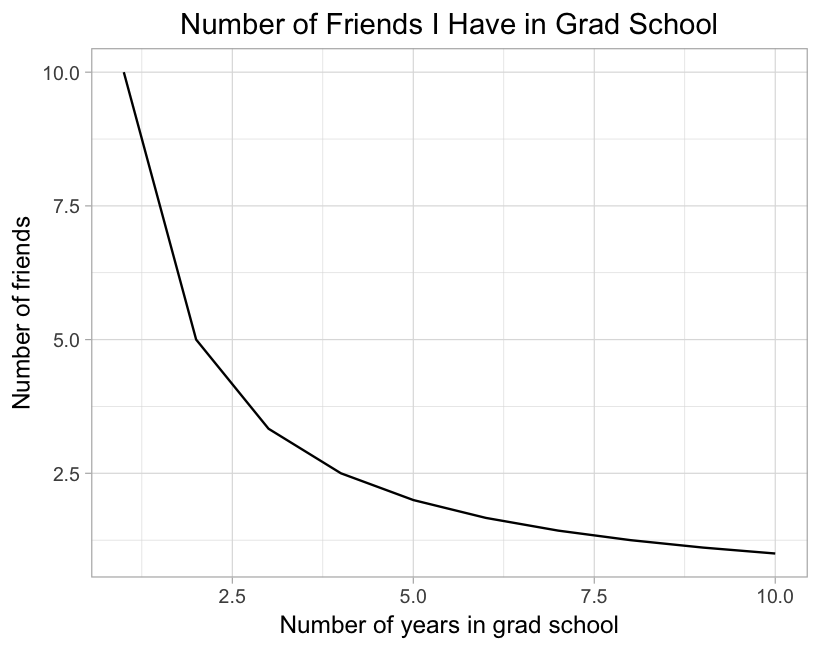
\includegraphics[scale=0.3]{friends}
    \caption{This is an example figure.}
    \label{fig:friends}
\end{figure}

\subsection{A Subsection}
\lipsum[2]
\subsubsection{A Subsubsection}
Table \ref{tbl:sepalwidth} summarizes the statistics. \lipsum[22] 

% latex table generated in R 3.5.0 by xtable 1.8-2 package
% Sat Aug 25 07:47:40 2018
\begin{table}[ht]
\centering
\begin{tabular}{rlrrrrr}
  \hline
 & Species & N & Sepal.Width & sd & se & ci \\ 
  \hline
1 & setosa & 50.00 & 3.43 & 0.38 & 0.05 & 0.11 \\ 
  2 & versicolor & 50.00 & 2.77 & 0.31 & 0.04 & 0.09 \\ 
  3 & virginica & 50.00 & 2.97 & 0.32 & 0.05 & 0.09 \\ 
   \hline
\end{tabular}
\caption{This is a table.}
\label{tbl:sepalwidth}
\end{table}

\subsection{A Second Subsection}
\lipsum[3]
\section{Section 2}
\lipsum[4]
\subsection{Another Subsection}
\lipsum[5-7]


 % Some chapter

\chapter{Background}

The graduate student consumes an increasing amount of coffee as the semester progresses (Figure \ref{fig:coffee}). \lipsum[2]

\begin{figure}[h]
    \centering
    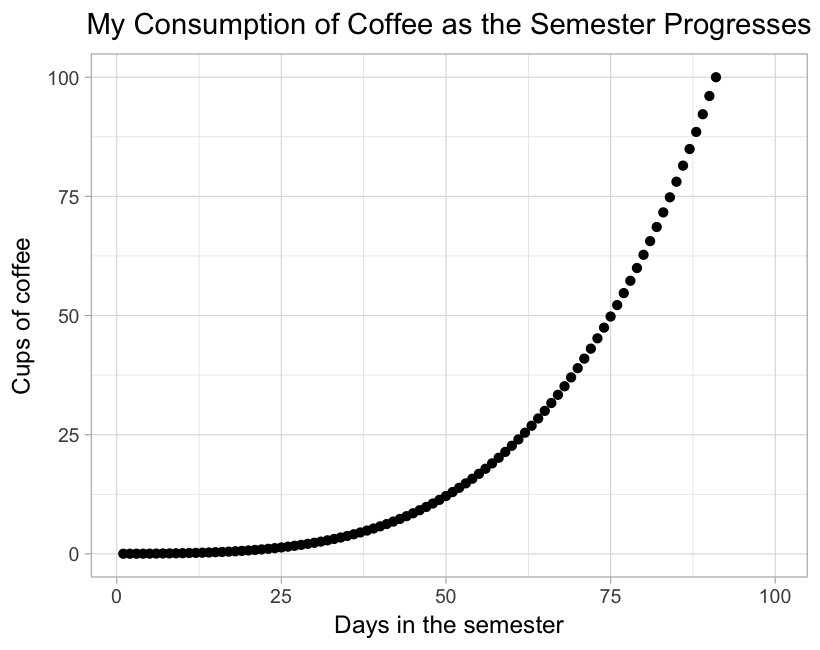
\includegraphics[scale=0.3]{coffee}
    \caption{This is an example figure.}
    \label{fig:coffee}
\end{figure} % Some chapter

\chapter{A really really really really really really really long chapter title}

\lipsum[3]

\begin{table}[h]
\centering
\begin{tabular}{|l|l|l|}
\hline
 o & x & o \\ \hline
 o & x & x  \\ \hline
 x & o & x \\ \hline
\end{tabular}
\caption{This is a second table.}
\end{table} % Some chapter

\chapter{Some chapter}

\lipsum[4] % Some chapter

%\chapter{Some chapter}

\lipsum[5] % Some chapter

%\chapter{Conclusion}

\lipsum[6] % Some chapter

\addtocontents{toc}{\vspace{2em}} 

\appendix

\chapter{An appendix}

\lipsum[81]

% latex table generated in R 3.5.0 by xtable 1.8-2 package
% Sat Aug 25 07:45:55 2018
\begin{table}[ht]
\centering
\begin{tabular}{rlrrrrr}
  \hline
 & Species & N & Sepal.Length & sd & se & ci \\ 
  \hline
1 & setosa & 50.00 & 5.01 & 0.35 & 0.05 & 0.10 \\ 
  2 & versicolor & 50.00 & 5.94 & 0.52 & 0.07 & 0.15 \\ 
  3 & virginica & 50.00 & 6.59 & 0.64 & 0.09 & 0.18 \\ 
   \hline
\end{tabular}
\caption{Oh look! It's a table.}
\end{table} % Appendix

\chapter{Another appendix}

% latex table generated in R 3.5.0 by xtable 1.8-2 package
% Sat Aug 25 08:04:38 2018
\begin{table}[ht]
\centering
\begin{tabular}{rrrrrr}
  \hline
 & mpg & cyl & disp & hp & drat \\ 
  \hline
Mazda RX4 & 21.00 & 6.00 & 160.00 & 110.00 & 3.90 \\ 
  Mazda RX4 Wag & 21.00 & 6.00 & 160.00 & 110.00 & 3.90 \\ 
  Datsun 710 & 22.80 & 4.00 & 108.00 & 93.00 & 3.85 \\ 
  Hornet 4 Drive & 21.40 & 6.00 & 258.00 & 110.00 & 3.08 \\ 
  Hornet Sportabout & 18.70 & 8.00 & 360.00 & 175.00 & 3.15 \\ 
  Valiant & 18.10 & 6.00 & 225.00 & 105.00 & 2.76 \\ 
  Duster 360 & 14.30 & 8.00 & 360.00 & 245.00 & 3.21 \\ 
  Merc 240D & 24.40 & 4.00 & 146.70 & 62.00 & 3.69 \\ 
  Merc 230 & 22.80 & 4.00 & 140.80 & 95.00 & 3.92 \\ 
  Merc 280 & 19.20 & 6.00 & 167.60 & 123.00 & 3.92 \\ 
  Merc 280C & 17.80 & 6.00 & 167.60 & 123.00 & 3.92 \\ 
  Merc 450SE & 16.40 & 8.00 & 275.80 & 180.00 & 3.07 \\ 
  Merc 450SL & 17.30 & 8.00 & 275.80 & 180.00 & 3.07 \\ 
  Merc 450SLC & 15.20 & 8.00 & 275.80 & 180.00 & 3.07 \\ 
  Cadillac Fleetwood & 10.40 & 8.00 & 472.00 & 205.00 & 2.93 \\ 
   \hline
\end{tabular}
\caption{Another table in another appendix.}
\label{tbl:mtcars}
\end{table} % Appendix

\addtocontents{toc}{\vspace{1em}}

% The bibliography
\clearpage
\addcontentsline{toc}{chapter}{Bibliography}
\bibliographystyle{apalike}
\bibliography{Bibliography} 

\end{document}